% !TEX root = ../main.tex
%
% ========
\chapter{Particle interferometry}
% ========
  Two-particle interferometry (also called \textit{femtoscopy}) gives a possibility to investigate space-time characteristics of the particle-emitting source created in heavy ion collisions.
  Through the study of particle correlations, their momentum distributions can be used to obtain information about the spatial extent of the created system.
  Using this method, one can measure sizes of the order of $10^{-15}$ m and time of the order of $10^{-23}$ s.
  %
  % ========
  \section{HBT interferometry}
  % ========
    In the 1956 Robert Hanbury Brown and Richard Q. Twiss proposed a method which through analysis of interference between photons allowed to investigate angular dimensions of stars.
    The most important result from the Hanbury-Brown-Twiss experiments is that two indistinguishable particles can produce an interference effect.
    There is almost no difference between normal interferometry and HBT method, except that the latter one does not take into account information about phase shift of registered particles.
    At the beginning this method was used in astronomy for photon interference, but this effect can be used also to measure extent of any emitting source.
    This method was adapted to heavy ion collisions to investigate dimensions of a system created in those collisions by studying correlations of identical particles~\cite{nonidfemto}.
    The main difference between HBT method in astronomy and femtoscopy is that the first one is based on space-time HBT correlations and the latter one uses momentum correlations.
    The momentum correlations yield the space-time picture of the source, whereas the space-time HBT correlations provide the characteristic relative momenta of emitted photons, which gives the angular size of the star without the knowledge of its radius and lifetime~\cite{florkowski}.
  % \section{Intensity interferometry in heavy ion collisions}
  %
  % ========
  \section{Theoretical approach}
  % ========
    Intensity interferometry in heavy ion physics uses similar mathematical formalism as the astronomy HBT measurement.
    Through the measurement of correlation between particles as a function of their relative momenta $\vect{q} = \vect{p_1} - \vect{p_2}$ one can deduce the average separation between emitting sources.
    %
    % ========
    \subsection{Two particle wave function}
    % ========
      Let us consider two identical particles with momenta $\vect{p_1}$ and $\vect{p_2}$ emitted from space points $\vect{x_1}$ and $\vect{x_2}$.
      Those emitted particles can be treated as two incoherent waves.
      \begin{figure}[h]
        \centering
        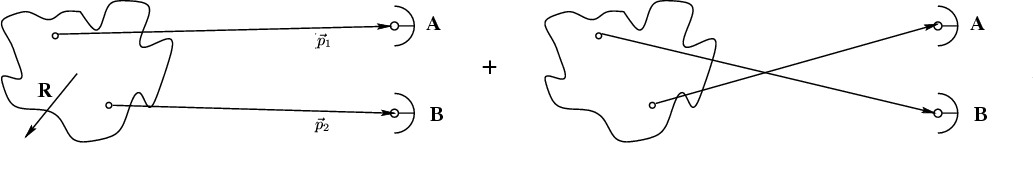
\includegraphics[width=0.9\textwidth]{wavefunction}
        \caption{The pair wave function is a superposition of all possible states. In case of particle interferometry it includes two cases: particles with momenta $p_1$,~$p_2$ registered by detectors \textit{A}, \textit{B} and $p_1$,~$p_2$ registered by \textit{B}, \textit{A} respectively.}
        \label{fig:wavefunction}
      \end{figure}
      If the particles are identical, they are also indistinguishable, therefore one has also take into account the scenario, where the particle with momentum $\vect{p_1}$ is emitted from $\vect{x_2}$ and particle $\vect{p_2}$ from $\vect{x_1}$ (Fig.~\ref{fig:wavefunction}).
      In such case, the wave function of a pair has to contain both components~\cite{drkisiel}:
      \begin{equation}
      \label{eq:wavefunction}
        \Psi_{ab}(\vect{q})=\frac{1}{\sqrt{2}} \left[ \exp(- i \vect{p_1}\vect{x_1} - i \vect{p_2}\vect{x_2}) \pm \exp(- i \vect{p_2}\vect{x_1} - i \vect{p_1}\vect{x_2}) \right]~.
      \end{equation}
      A two particle wave function of identical bosons is symmetric (``+'' sign in Eq.~\ref{eq:wavefunction}) and in case of identical fermions - antisymmetric (``-'' sign).
      This anti-symmetrization or symmetrization implies the correlation effect coming from the Fermi-Dirac or Bose-Einstein statistics accordingly.

      To provide full description of a system consisting of two charged hadrons, one has to include in the wave function besides quantum statistics also Coulomb and strong Final State Interactions.
      Considering identical particles systems, the quantum statistics is a main source of a correlation.
      In case of space-time analysis of particle emitting source, effects coming from the Coulomb and Strong interactions are negligible.

    %
    % ========
    \subsection{Source function}
    % ========

    %
    % ========
    \subsection{Theoretical correlation function}
    % ========

    %
    % ========
    \subsection{Spherical harmonics decomposition of a correlation function}
    % ========
  %
  % ========
  \section{Experimental approach}
  % ========

  % include drkisiel p. 35?

  %
  % ========
  \section{Scaling of femtoscopic radii}
  % ========
